%!TEX root = ../main.tex

\section{Decay time fit}
\label{sec:b02dd:decaytimefit}

The conditional PDF describing the reconstructed decay time $t'$ and tag
decisions $\vect{d'} = (\dos, \dss)$, given a per-event decay time resolution
$\sigma_{t'}$ and per-event mistag probability estimates $\vect{\eta} = (\etaos,
\etass)$, is
%
\begin{equation}\label{eq:fullpdf}
  P\left(t',\vect{d'}\given \sigma_{t'},\vect{\eta}\right)
  \propto \epsilon(t') \left(\mathcal{P}(t,\vect{d'}\given \vect{\eta})
    \otimes \mathcal{R}(t'-t\given \sigma_{t'})\right)\,,
\end{equation}
%
where
\begin{equation}
  \mathcal{P}(t,\vect{d'}\given \vect{\eta}) \\
  \propto \sum_{d} \mathcal{P}(\vect{d'} \given d,\vect{\eta})
      [1 - d\, A_\text{P}] \,
      e^{-t/\tau}\left\{1 - d\, S \sin(\dm t) + d\, C \cos(\dm t)\right\}\,,
\end{equation}
and where $t$ is the true decay time, $d$ is the true production flavour,
$A_\text{P}$ is the production asymmetry, and $\mathcal{P}(\vect{d'} \given
d,\vect{\eta})$ is a two-dimensional binomial PDF describing the distribution
of tagging decisions given $\vect{\eta}$ and $d$. Normalisation factors are omitted for brevity.

%============================================================================%
%!TEX root = ../main.tex
\section{Decay time resolution}
\label{sec:dataanalysis::resolution}

Uncertainties in the determination of the position of vertices and in the
measurement of momenta (although thanks to the VELO (see
\cref{sec:detector:lhcb}) pretty accurate  at $\lhcb$) lead to a finite decay
time resolution $\sigma$, which dilutes the observed $\CP$ asymmetry by a
factor
\begin{align}
  \mathcal{D} = e^{\frac{-\dmd^2\,\sigma^2}{2}} \, .
\end{align}
This formula is the special case for a Gaussian resolution model with width
$\sigma$. The general formula is derived in
Ref.~\cite{ResolutionDilutionFactor}. For $\Bd$ mesons the dilution induced by
the decay time resolution has only minor influence on the measurement of $\CP$
observables because the oscillation frequency of $\Bd$ mesons $\dmd =
\SI{0.5064\pm0.0019}{\hbar\invps}$~\cite{HFAG} is quite low. Even for a decay time
resolution of \SI{100}{\fs}, which would be almost two times larger than what
is usually found in analyses performed by \lhcb, the dilution factor is
greater than \SI{99}{\percent}.

\FloatBarrier
%============================================================================%
%!TEX root = ../main.tex
\subsection{Decay time acceptance}
\label{sec:b02dd:decaytimefit:acceptance}

The trigger requirements as well as some input variables to the BDT result in
a decay-time-dependent efficiency. Additionally, the \velo reconstruction
(\ie the FastVelo algorithm~\cite{Callot:2011bza}) causes a drop in decay time
acceptance for events with large decay times. In order to correctly describe
these effects the $\Bd$ lifetime is constrained to its PDG value of $\tau =
\SI{1.519\pm0.005}{\ps}$~\cite{PDG2014} in the nominal fit and any deviation
of the decay time distribution (summed over the tags) from a pure exponential
shape is supposed to be described by cubic splines (see
\cref{sec:dataanalysis:splines}). Knots are positioned on the rising edge,
approximately at the turning point, and at the boundaries of the decay time
range, so at $\{\SIlist[list-final-separator={,
}]{0.25;0.8;2.0;10.25}{\ps}\}$. The normalisation of the splines is arbitrary
and it has been decided to fix the second to last spline coefficient to
$\num{1.0}$.

On signal MC the truth information is available so the shape of the decay time
acceptance can be separated from the exponential decay. This shape is compared
with the spline method described above. As the BDTs are trained and applied
separately for the two final states and might have different effects on the
shape of the decay time acceptance these two categories are studied
individually.

\begin{figure}[htb]
\centering
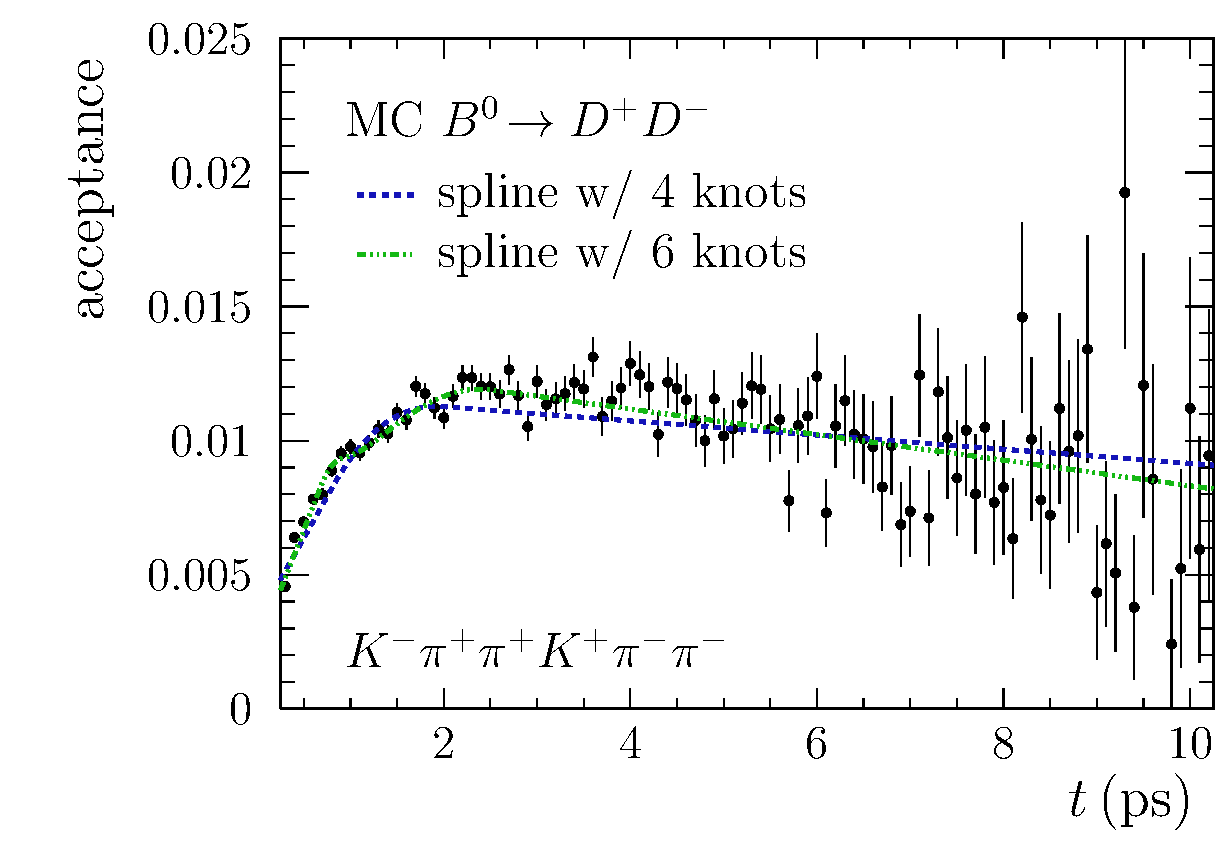
\includegraphics[width=0.48\textwidth]{07-B02DD/tikz/pdf/Acceptancespline_nolog_MC_Kpipi.pdf}
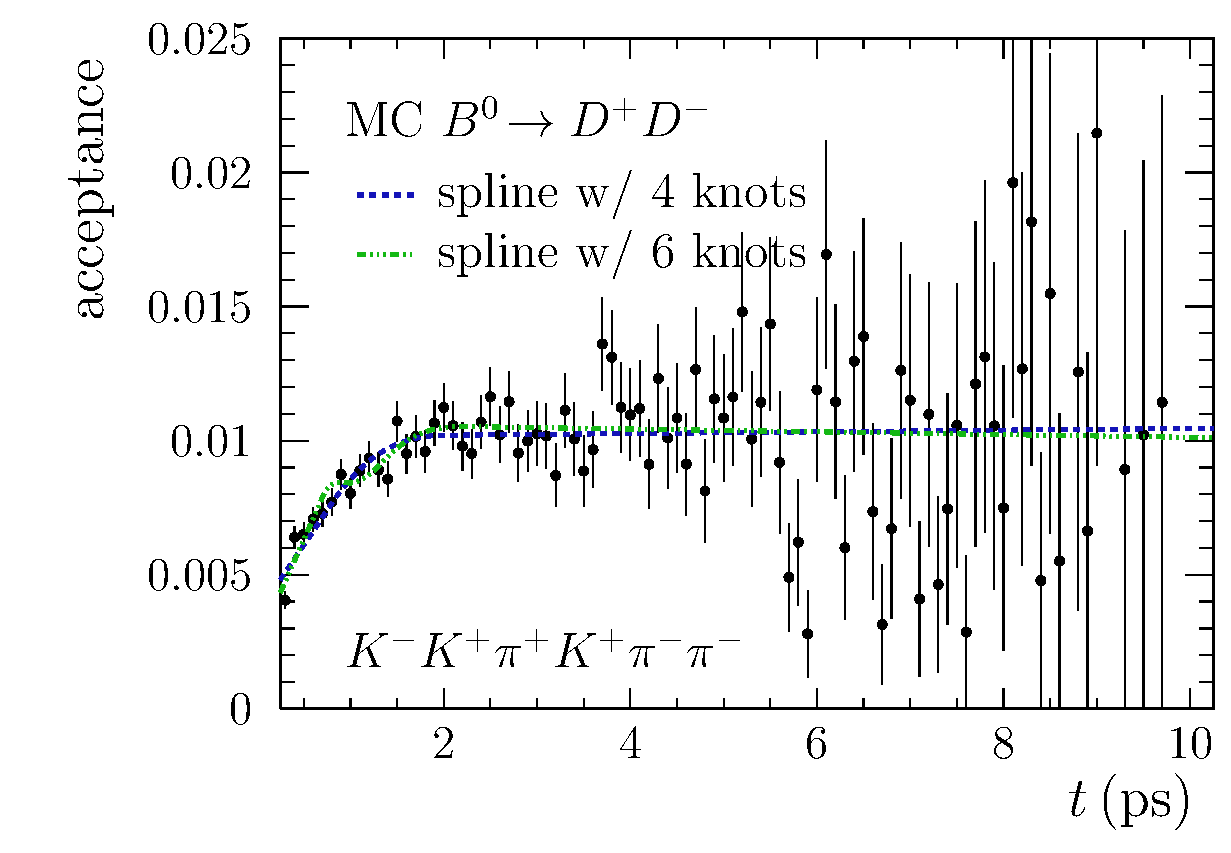
\includegraphics[width=0.48\textwidth]{07-B02DD/tikz/pdf/Acceptancespline_nolog_MC_KKpi.pdf}
\caption{Decay time acceptance of truth-matched signal MC for the $\KpipiKpipi$
final state (left) and the $\KKpiKpipi$ final state (right). The black data
points show the true decay time acceptance determined by dividing the
reconstructed by the true decay time distribution. The blue line is the spline
acceptance function and the red stripes indicate the $1\,\sigma$ error band
taking into account the statistical uncertainties.}
\label{fig:b02dd:decaytimefit:acceptance_MC}
\end{figure}

Looking at the plots in \cref{fig:b02dd:decaytimefit:acceptance_MC} it is
apparent that compared to $\BdToJPsiKS$ there is a quite large efficiency loss
at high decay times. This might be related to the fact that both $\Bd$
daughter particles ($\Dp$ and $\Dm$) are relatively long-lived. The true MC
decay time acceptance is overlaid with the shape of two spline functions.
Besides the spline function with the nominal number of four knots an
additional spline function with two more knots and slightly changed positions
$(\SIlist[list-final-separator={, }]{0.25;0.7;1.0;1.5;2.5;10.25}{\ps})$ is
plotted, which gives a better description. But it has to be considered that
the statistics of the MC sample is \num{25} times larger than the real data.
Therefore, the spline function with four knots is chosen, otherwise rather
statistical fluctuations than acceptance effects would be described. The low
statistics of the $\KKpiKpipi$ final state on real data does also not allow to
use separate spline coefficients for the two final states although with the
increased MC statistics some differences become visible.


\FloatBarrier
%============================================================================%
\subsection{External inputs}
\label{sec:b02dd:decaytimefit:constraints}

\lhcb has performed a measurement of the production asymmetry as a function
of transverse momentum and pseudorapidity using \SI{7}{\TeV}
data~\cite{LHCb-PAPER-2014-042}. Taking those distributions from \BdToDD
individual weighted averages for the 2011 and 2012 subsamples are calculated
yielding
%
\begin{equation}
  \begin{split}
    \prodasym{11} &= -0.0047 \pm 0.0106 \,\text{(stat)} \pm 0.0014 \, \text{(syst)} \,, \\
    \prodasym{12} &= -0.0071 \pm 0.0107 \,\text{(stat)} \pm 0.0014 \, \text{(syst)} \,.
  \end{split}
\end{equation}
%
As the measurement of the production asymmetry has been performed on 2011 data
only, the numbers for $\prodasym{11}$ and $\prodasym{12}$ are highly
correlated. So, the latter is modelled as $\prodasym{12} = \prodasym{11} +
\Delta\prodasym{}$ with $\Delta\prodasym{} = -0.0024 \pm 0.0018
\,\text{(syst)}$. The systematic uncertainty accounts for the difference of
the production asymmetries observed for the two data-taking conditions in the
measurement of the semileptonic $\CP$ asymmetry~\cite{LHCb-PAPER-2014-053} and
is used as width of a Gaussian constraint. The $\Bz$ oscillation frequency and
the $\Bz$ lifetime are constrained to their world averages $\dm =
\SI{0.510\pm0.004}{\planckbar\invps}$~\cite{HFAG} and $\tau =
\SI{1.519\pm0.005}{\ps}$~\cite{PDG2014}, respectively. The decay time
resolution parameters (\cref{tab:b02dd:decaytimefit:resolution}), the flavour
tagging calibration parameters
(\cref{tab:dataanalysis:taggingcalibration:dsdcalibration}), which are taken
from the \BdToDsD calibration, and the $\Bz$ lifetime difference $\DG =
\SI{0}{\invps}$ are fixed in the likelihood fit.

%============================================================================%
\subsection{Results}

\todo{consider which uncertainties should be quoted, full FT uncertainties in constraints?}
The fit results of the $\CP$ observables from the decay time fit are
\begin{align}
\begin{split}
  \SDD                &= -0.54\,\pm\,0.17 \, , \\
  \CDD                &= \phantom{-}0.26\,\pm\,0.17 \, , \\
  \rho(\SDD,\CDD)     &= \phantom{-}0.48 \, . \\
\end{split}
\label{eq:b02dd:decaytimefit:cpresults}
\end{align}

Only after rescaling the sWeights via
\begin{align}
  w_i = w_i \frac{\sum w_i}{\sum w_i^2}\,,
\end{align}
correct asymmetric uncertainty estimates are delivered by \minos, which is
\root's standard method to analyse the likelihood shape. To check if the
coverage is guaranteed the bootstrapping method is applied. The nominal fit
procedure, \ie performing the mass fit, calculating the sWeights and fitting
the weighted tagged decay time distribution, is executed and the fit results
are stored. The drawing and fitting is done \num{10000} times. It turns out
that half of the fits fail if the flavour tagging calibration parameters are
constrained within their statistical uncertainties. When fixing them to their
central values the fit failure rate drops to a per-mille effect. From the
distribution of fit results the two-side \SI{68}{\percent} confidence
intervals are extracted. To account for the uncertainties on the flavour
tagging calibration parameters \num{10000} pseudoexperiments are performed, in
which the nominal model is used to generate the signal decay time distribution
and the fit results of the nominal fit are chosen for the \CP observables \SDD
and \CDD. Before generating the flavour tagging calibration parameters are
drawn from Gaussian distributions around their central values using the
combined statistical + systematic uncertainties. In the subsequent fit the
flavour tagging calibration parameters are fixed to their central values, like
in the fits to the bootstrapped samples. The resulting pull distributions are
broader than standard normal distributions. The deviation of the width from
unity shows how much the statistical uncertainties are underestimated in the
likelihood fit due to not accounting for the variation of the flavour tagging
calibration parameters. So, the statistical uncertainties for \SDD and
\CDD from the bootstrapping including the impact of the uncertainty of the
flavour tagging calibration parameters are given by scaling the bootstrapping
uncertainties by the width of the pull distributions:
\begin{align}
    \sigma_{\SDD}(\text{bootstrapping}) &= \,^{+0.17}_{-0.16} \,, \\
    \sigma_{\CDD}(\text{bootstrapping}) &= \,^{+0.18}_{-0.17} \,.
\end{align}
These uncertainties match the nominal ones from \minos quite well. A plot of
the decay time distribution and the projection of the acceptance model are
shown in \cref{fig:b02dd:decaytimefit}. Good agreement between the latter and
the shape on signal MC (cf. \cref{fig:b02dd:decaytimefit:acceptance_MC}) can
be observed but the low statistics leading to rather large uncertainties
indicated by the error band diminishes the significance of the comparison.

\begin{figure}[htb]
\hspace*{\fill}
\begin{minipage}{0.4\textwidth}
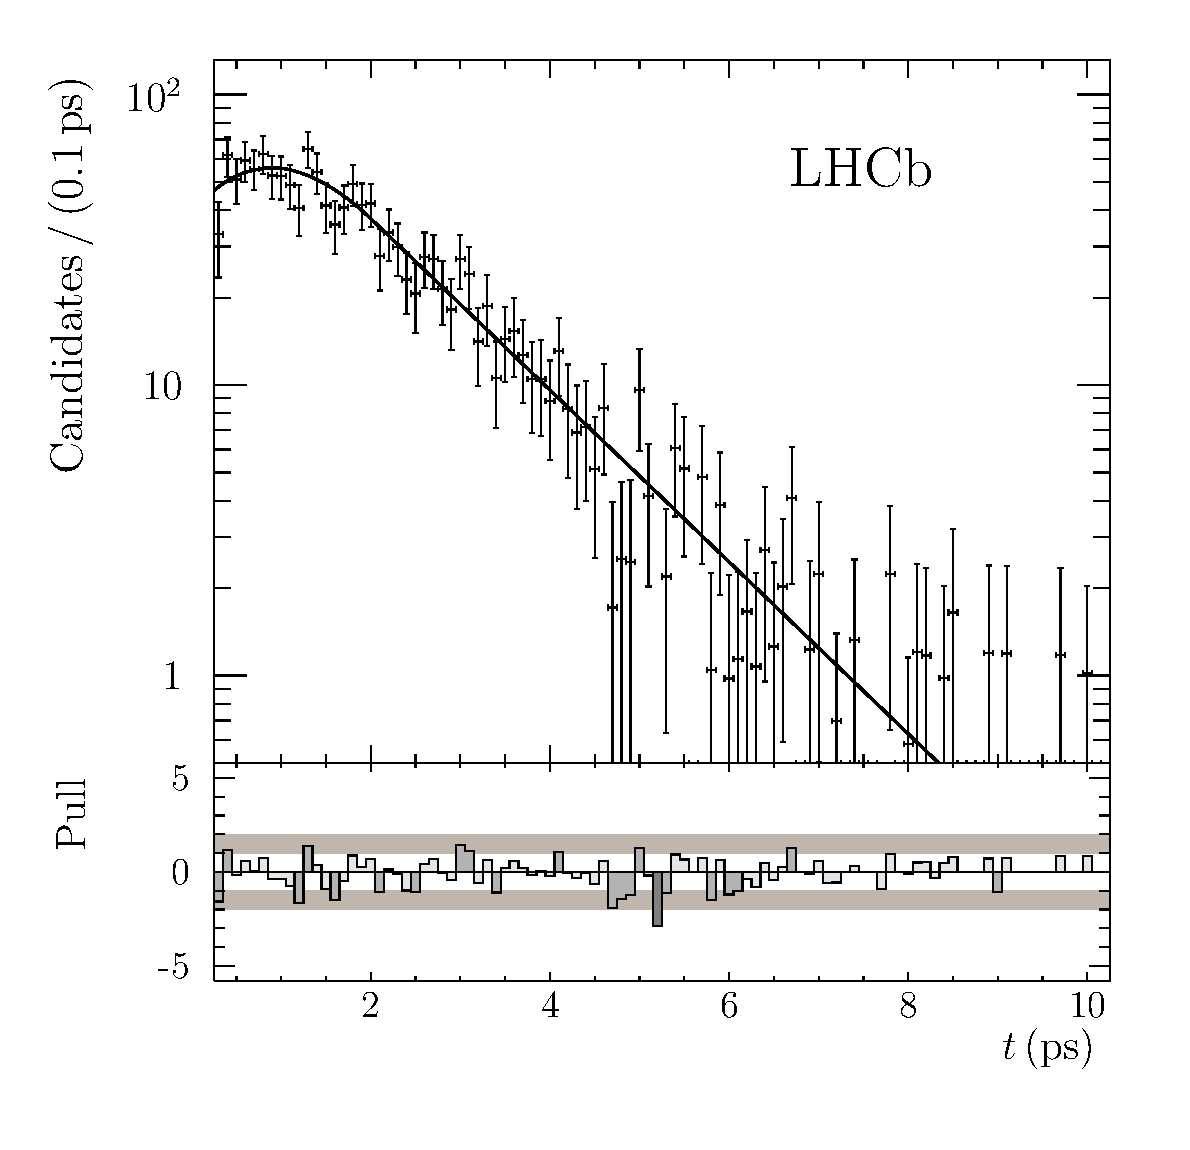
\includegraphics[width=\textwidth]{07-B02DD/tikz/pdf/obsTime_summed_pull_logy.pdf}
\end{minipage}
\hfill
\begin{minipage}{0.5\textwidth}
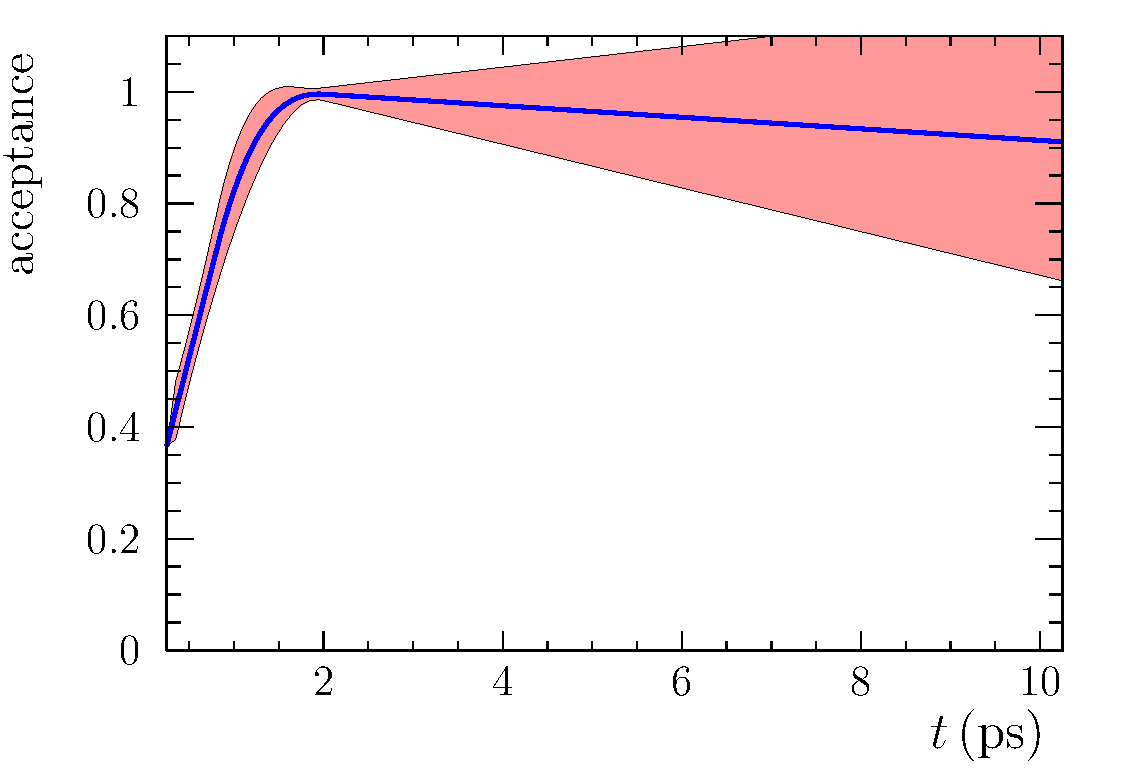
\includegraphics[width=\textwidth]{07-B02DD/tikz/pdf/Acceptancespline_nolog.pdf}
\end{minipage}
\hspace*{\fill}
\caption{Plot of the decay time distribution of the background-subtracted \BdToDD
data sample with the projection of the \PDF and the pull distribution on the
left. The y-axis is plotted in logarithmic scale. Plot of the nominal decay
time acceptance model on the right. The red area indicates the 1\,$\sigma$
error band taking into account the statistical uncertainties.}
\label{fig:b02dd:decaytimefit}
\end{figure}

Apart from a quite high positive correlation between the parameters of the
acceptance spline function and the already quoted correlation of about
\num{0.5} between $\SDD$ and $\CDD$, which is expected from first principles
(see Ref.~\cite{LHCb-ANA-2011-004}), no large correlation between fitted parameters
is present as can be seen from the correlation matrix visualised in
\cref{fig:b02dd:decaytimefit:FullFitCorrMatrixHotCold}. A possible correlation
between $\dm$ and $\CDD$ is significantly reduced by the constraint applied on $\dm$,
which is a lot tighter than the sensitivity accessible from the data sample.
When releasing this constraint the correlation coefficient becomes \num{-0.8}.
But the sensitivity on $\CDD$ would significantly go down in this scenario so
the constraint on $\dm$ is maintained in the nominal setup.

\begin{figure}[htb]
\centering
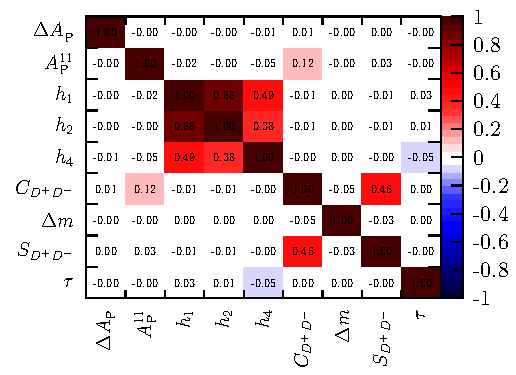
\includegraphics[width=0.5\textwidth]{07-B02DD/tikz/pdf/FitResultsCorrMatrix_RedBlueDiscrete_wText.pdf}
\caption{Visualised correlation matrix of the fit parameters in the decay time
fit to data. Positive correlations are represented by the red palette on the $z$ axis,
while negative correlations are represented by the blue palette of the $z$
axis.}
\label{fig:b02dd:decaytimefit:FullFitCorrMatrixHotCold}
\end{figure}

The 1D likelihood scans in \cref{fig:b02dd:decaytimefit:1DLLScan} show a nice
parabolic shape with a clear minimum.
\begin{figure}[htb]
\centering
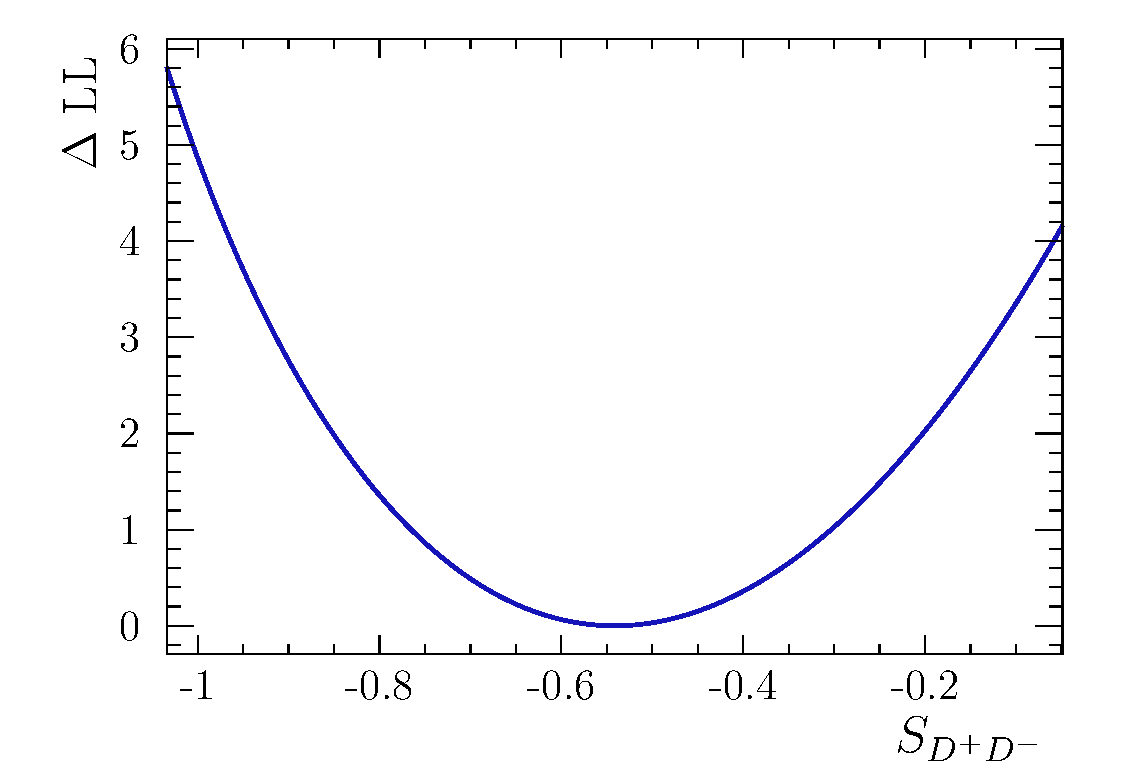
\includegraphics[width=0.48\textwidth]{07-B02DD/tikz/pdf/Likelihoodscan_sin2b.pdf}
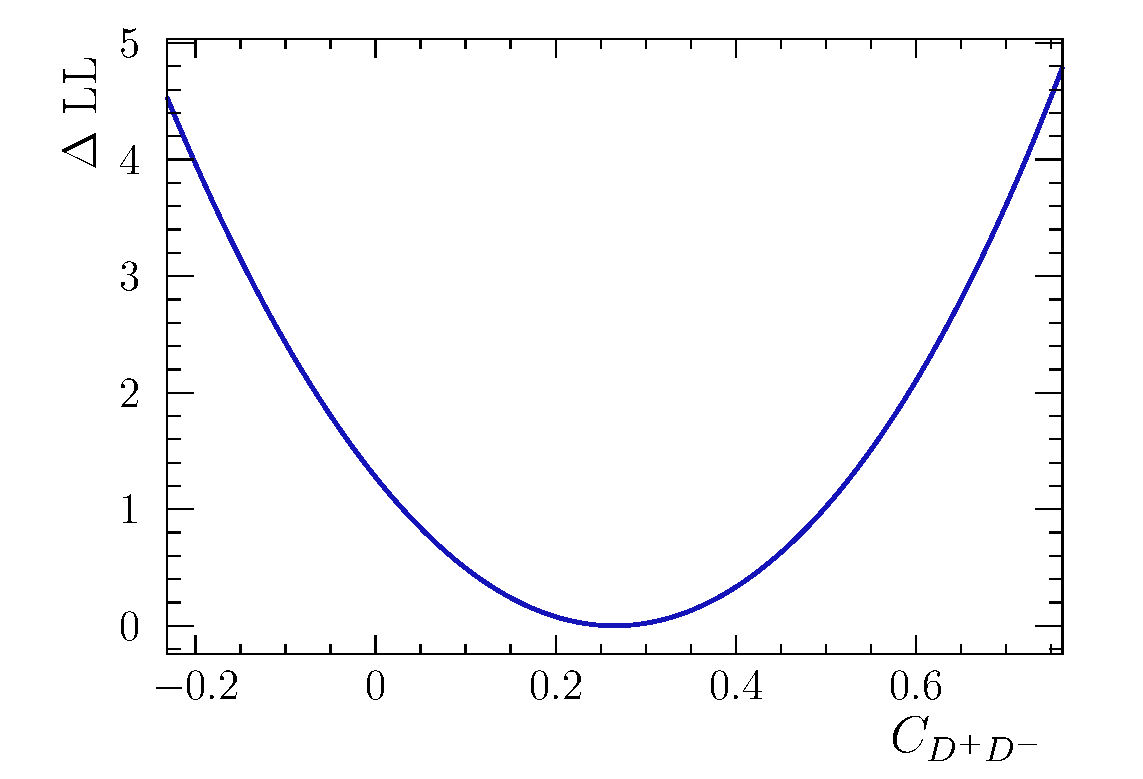
\includegraphics[width=0.48\textwidth]{07-B02DD/tikz/pdf/Likelihoodscan_C.pdf}
\caption{One-dimensional likelihood profile scans for $\SDD$ and $\CDD$.}
\label{fig:b02dd:decaytimefit:1DLLScan}
\end{figure}

% The 2D likelihood scan is depicted in \cref{fig:b02dd:decaytimefit:2DLLScan}.
% \begin{figure}[tb]
% \centering
% % \includegraphics[width=0.48\textwidth]{07-B02DD/figs/2DLikelihoodscan.pdf}
% \caption{Two dimensional likelihood profile scan for $\SDD$ and $\CDD$.
% The contour line shows the $1\sigma$ confidence level.}
% \label{fig:b02dd:decaytimefit:2DLLScan}
% \end{figure}

In \cref{fig:b02dd:decaytimefit:asymmetry} the signal yield asymmetry is
plotted in eight bins of the decay time. A binned $\chisq$-fit to this signal
asymmetry is performed using
\begin{align}
{\mathcal A}^{\text{meas}}(t) = \frac{\Delta\omega + \prodasym{11}(1 - \Delta\omega) + (1 - \Delta\omega + \prodasym{11}\Delta\omega){\mathcal A}^{\text{theo}}(t)}{1 + \prodasym{11}(\SDD \sin(\dm\,t) - \CDD \cos(\dm\,t))}\,,
\label{eq:b02dd:decaytimefit:asymmetry_td}
\end{align}
which is a modified version of the theoretical signal asymmetry in
\cref{eq:cpviolation:asymmetry} and accounts for the asymmetries induced by
flavour tagging ($\Delta\omega$) and production asymmetry ($\prodasym{11}$).
The fit results
\begin{align*}
\begin{split}
  \SDD                &= -0.65\,\pm\,0.25 \,, \\
  \CDD                &= \phantom{-}0.24\,\pm\,0.26 \,,
\end{split}
\end{align*}
are compatible with those from the unbinned fit presented in
\cref{eq:b02dd:decaytimefit:cpresults} but not as sensitive.
\begin{figure}[htb]
\centering
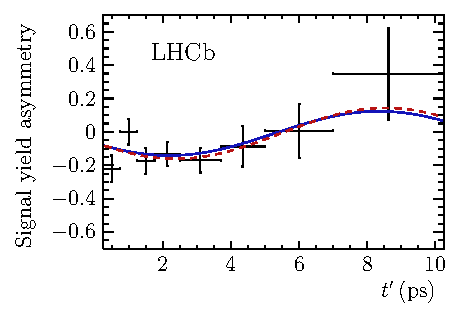
\includegraphics[width=0.48\textwidth]{07-B02DD/tikz/pdf/Asymmetry.pdf}
\caption{Decay-time-dependent signal yield asymmetry. The solid blue curve is the
projection of the signal PDF given in \cref{eq:fullpdf} and the dashed red curve is the
pure time-dependent fit function from
\cref{eq:b02dd:decaytimefit:asymmetry_td}}
\label{fig:b02dd:decaytimefit:asymmetry}
\end{figure}

\FloatBarrier
